\chapter{Limitaciones}
\label{cap:limitaciones}

\opening{Los límites no son metas: son el borde a partir del cual el metal empieza a acumular daño invisible.}

\section{Generalidades}

Este capítulo reúne las limitaciones de operación, las marcas de los instrumentos y los letreros básicos requeridos para la operación segura del helicóptero, su motor y los sistemas estándar. El helicóptero está aprobado como giroavión de categoría normal bajo el Certificado Tipo FAA H10WE en los modelos R22, R22 Alpha, R22 Beta y R22 Mariner.\fuente{POH, sección 2 (aprobada por la FAA), con las revisiones del 22 FEB 2024}

\section{Código de colores de los instrumentos}

\begin{checklist}
\chk{Rojo}{Límite de operación. El borde de la línea roja indica el límite; la aguja no debe entrar en el rojo en operación normal.}
\chk{Amarillo}{Rango de precaución o de procedimiento especial.}
\chk{Verde}{Rango normal de operación.}
\end{checklist}

\section{Límites de velocidad}

\textbf{Velocidad que nunca debe excederse (\textsc{v}\textsubscript{NE}):} 102~KIAS hasta 3000~ft de altitud de densidad. Sobre 3000~ft de altitud de densidad, la \textsc{v}\textsubscript{NE} disminuye según los letreros de la sección~\ref{sec:letreros-vne}.

\section{Límites de RPM del rotor}

\begin{table}[htbp]
\centering\small
\caption{Límites de RPM del rotor principal.}
\begin{tabular}{@{}lcc@{}}
\toprule
Condición & Máximo & Mínimo \\
\midrule
Con potencia & 104\,\% (530 RPM) & 101\,\% (515 RPM)\textsuperscript{a,b} \\
Sin potencia (autorrotación) & 110\,\% (561 RPM) & 90\,\% (459 RPM) \\
\bottomrule
\end{tabular}

\smallskip
\begin{minipage}{.92\linewidth}\footnotesize
\textsuperscript{a} Se permite operación transitoria a RPM más baja para el entrenamiento de procedimientos de emergencia.\\
\textsuperscript{b} Se permite 97\,\% (495 RPM) en los R22 con motor O-320 y tacómetro con arco verde de 97 a 104\,\%.
\end{minipage}
\end{table}

\section{Limitaciones del grupo motor}

\textbf{Motor:} un Lycoming modelo O-320-A2B, -A2C, -B2C u O-360-J2A.

\begin{table}[htbp]
\centering\small
\caption{Límites de operación del motor.}
\begin{tabularx}{\linewidth}{@{}Yr@{}}
\toprule
Parámetro & Límite \\
\midrule
RPM de motor, máxima continua & 104\,\% (2652 RPM) \\
RPM de motor, máxima transitoria\textsuperscript{*} & 106\,\% (2700 RPM) \\
Temperatura máxima de culata (CHT) & 500~°F (260~°C) \\
Temperatura máxima de aceite & 245~°F (118~°C) \\
Presión de aceite mínima en ralentí & 25 psi \\
Presión de aceite mínima en vuelo & 55 psi \\
Presión de aceite máxima en vuelo & 95 psi \\
Presión de aceite máxima en arranque y calentamiento & 115 psi \\
Cantidad mínima de aceite para despegue & 4 qt (3,8 l) \\
Presión de admisión & Según letreros (sección~\ref{sec:letreros-map}) \\
\bottomrule
\end{tabularx}

\smallskip
\begin{minipage}{.92\linewidth}\footnotesize
\textsuperscript{*} Está prohibida la operación intencional por encima de la velocidad máxima continua.
\end{minipage}
\end{table}

\section{Límites de peso}

\begin{checklist}
\chk{Peso bruto máximo --- Standard y HP}{1300 lb (590 kg)}
\chk{Peso bruto máximo --- Alpha, Beta y Beta II}{1370 lb (622 kg)}
\chk{Peso bruto mínimo}{920 lb (417 kg)}
\chk{Máximo por asiento, incluido su compartimiento de equipaje}{240 lb (109 kg)}
\chk{Máximo en cualquiera de los compartimientos de equipaje}{50 lb (23 kg)}
\end{checklist}

\section{Límites del centro de gravedad}

El dato de referencia está 100~in por delante del eje del rotor principal. Los límites longitudinales y laterales se muestran en las figuras~\ref{fig:cg-std} y~\ref{fig:cg-beta}.

\begin{nota}
Con ambas puertas instaladas, un piloto solo con un peso (incluido su equipaje) de 135~lb (61~kg) o más asegura que el CG quede dentro de límites. Con pesos menores, calcule el peso y balance; puede requerirse lastre removible para llevar el CG a la posición del límite trasero o por delante de él (ver el capítulo~\ref{cap:peso-balance}).
\end{nota}

\begin{figure}[htbp]
\centering
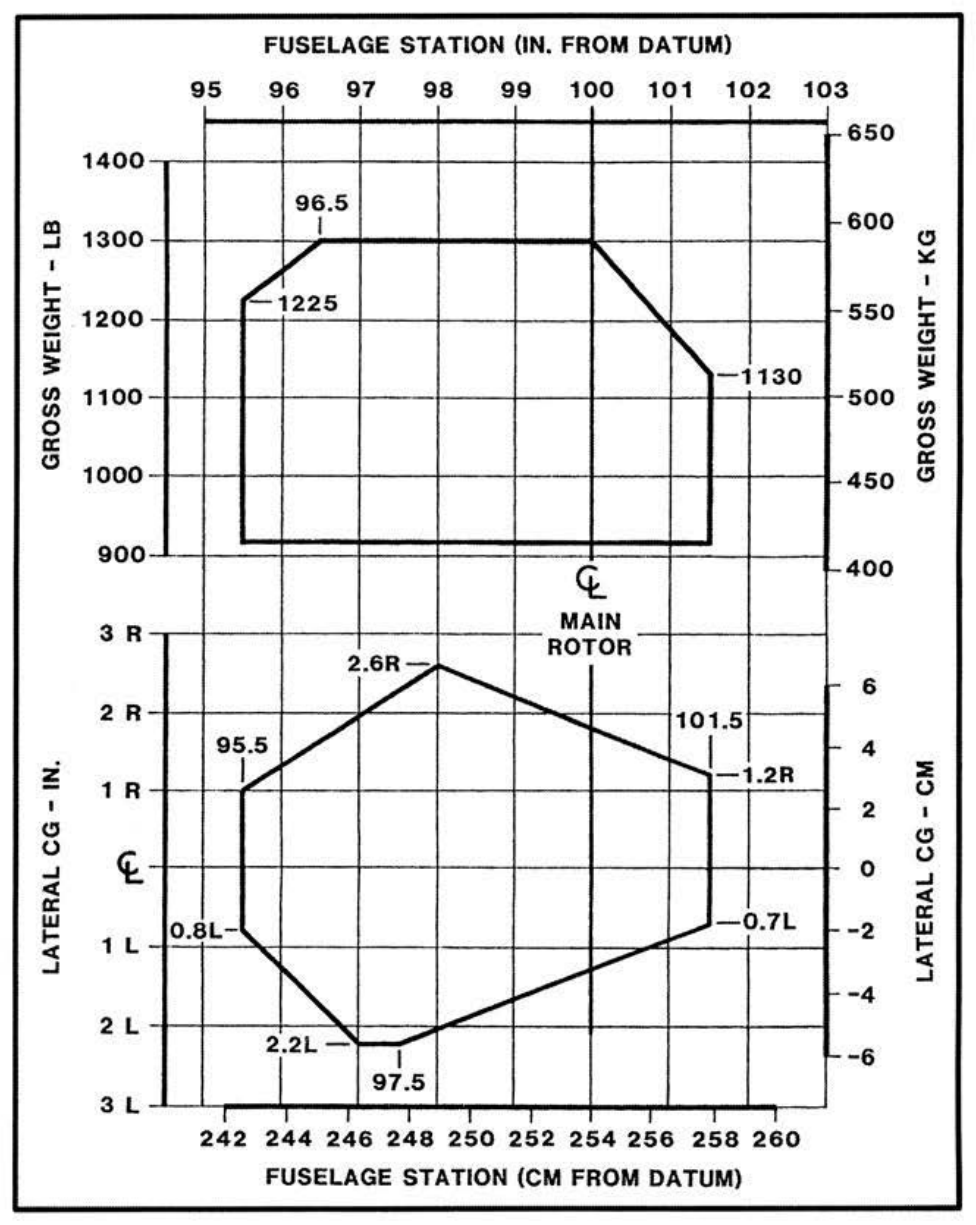
\includegraphics[width=.8\linewidth]{assets/poh/cg-standard.png}
\caption{Límites de CG del R22 Standard y HP. Longitudinal: límite delantero 96,5~in a 1300~lb y 95,5~in a 1225~lb o menos; límite trasero 100,0~in a 1300~lb y 101,5~in a 1130~lb o menos. Lateral: de 2,2~in a la izquierda (L) a 2,6~in a la derecha (R) según la estación.}
\label{fig:cg-std}
\end{figure}

\begin{figure}[htbp]
\centering
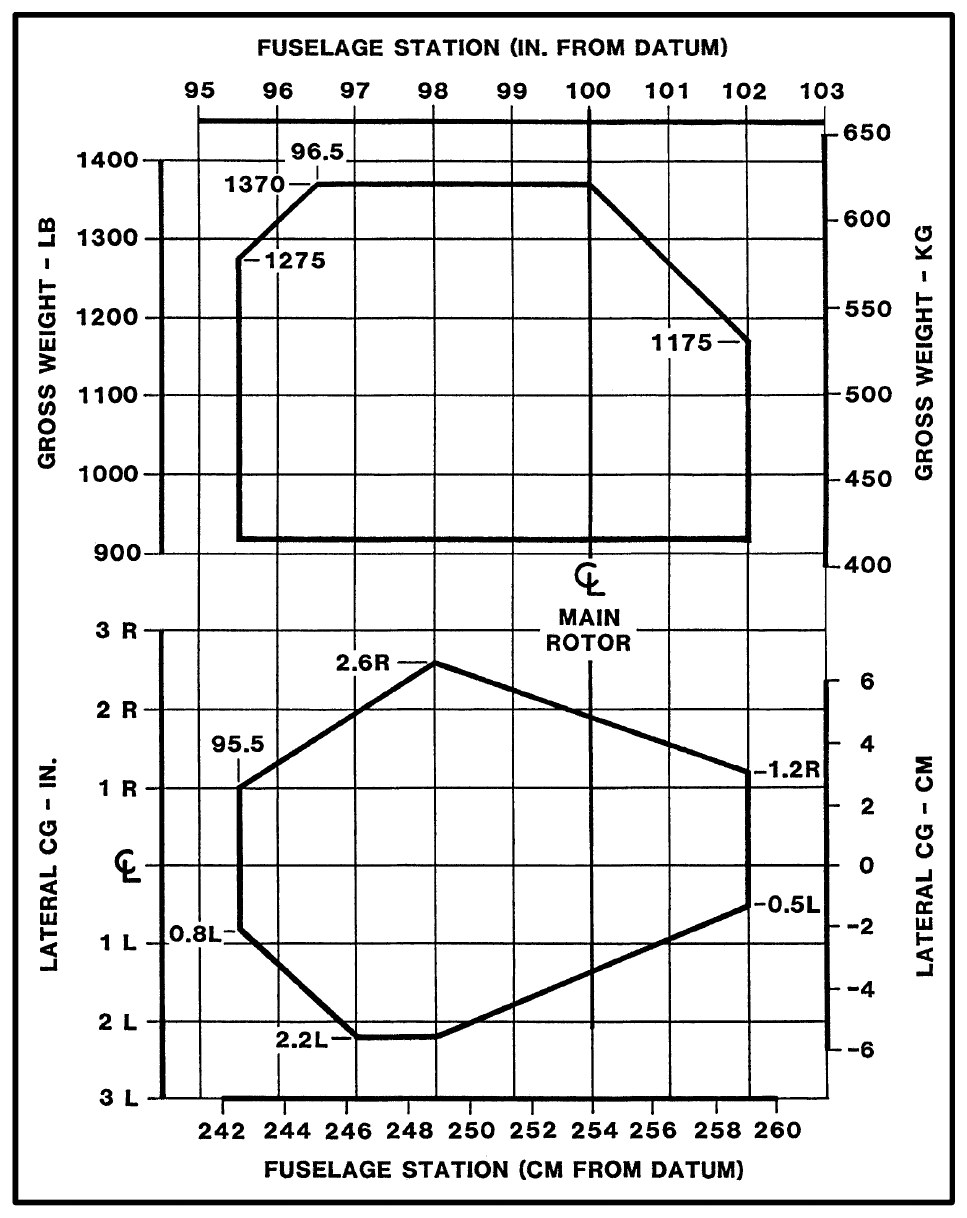
\includegraphics[width=.8\linewidth]{assets/poh/cg-alpha-beta.png}
\caption{Límites de CG del R22 Alpha, Beta y Beta II. Longitudinal: límite delantero 96,5~in a 1370~lb y 95,5~in a 1275~lb o menos; límite trasero 100,0~in a 1370~lb, que se desplaza hacia atrás hasta su posición más retrasada a 1175~lb o menos. Lateral: entre 2,2~in L y 2,6~in R según la estación.}
\label{fig:cg-beta}
\end{figure}

\section{Limitaciones de vuelo y maniobra}

\begin{itemize}
\item Prohibido el vuelo acrobático.
\end{itemize}

\begin{precaucion}
Las acciones bruscas sobre los controles pueden producir altas tensiones de fatiga y causar la falla catastrófica de un componente crítico.
\end{precaucion}

\begin{itemize}
\item Prohibidos los empujes de cíclico en baja G (\emph{low-G pushovers}).
\end{itemize}

\begin{precaucion}
Un empuje (maniobra de cíclico adelante) efectuado desde vuelo nivelado o después de un tirón hacia arriba produce una condición de baja G (casi ingravidez) que puede causar la pérdida catastrófica del control lateral. Para eliminar una condición de baja G, aplique de inmediato cíclico atrás suave. Si se inicia un alabeo durante una condición de baja G, aplique cíclico atrás suave para volver a cargar el rotor \emph{antes} de aplicar cíclico lateral para detener el alabeo.
\end{precaucion}

\begin{itemize}
\item Prohibido el vuelo con el gobernador desconectado, salvo ante una falla de sistemas en vuelo o durante el entrenamiento de procedimientos de emergencia.
\item Prohibido el vuelo en condiciones de engelamiento conocidas.
\item Altitud de densidad máxima de operación: 14\,000~ft.
\item El alternador, el gobernador de RPM, el sistema de aviso de baja RPM del rotor y el indicador de OAT deben estar operativos para el despacho.
\item La tripulación mínima es un piloto en el asiento derecho. Un instructor de vuelo puede actuar como piloto al mando desde el asiento izquierdo.
\item Vuelo solo únicamente desde el asiento derecho.
\item El cinturón del asiento izquierdo debe estar abrochado.
\item Se aprueba la operación con una o ambas puertas de cabina removidas. Durante el vuelo sin puertas, los objetos sueltos en la cabina deben estar debidamente asegurados.
\item Cada piloto debe usar un audífono (\emph{headset}) en funcionamiento.
\end{itemize}

\section{Limitaciones por tipo de operación}

Se aprueban operaciones VFR diurnas y nocturnas. El VFR nocturno se permite solo con las luces de aterrizaje, de navegación, de instrumentos y anticolisión operativas. La orientación durante el vuelo nocturno debe mantenerse por referencia visual a objetos del terreno iluminados solamente por luces en tierra o por una iluminación celeste adecuada.

\begin{nota}
Pueden existir requisitos adicionales en países distintos de los Estados Unidos.
\end{nota}

\section{Limitaciones de combustible}

\subsection{Grados de combustible aprobados}

\begin{table}[htbp]
\centering\small
\caption{Grados de combustible aprobados.}
\begin{tabularx}{\linewidth}{@{}lL{2.2cm}Y@{}}
\toprule
Grado & Color & Especificación \\
\midrule
100 & Verde & \multirow{3}{*}{ASTM D910} \\
100LL & Azul & \\
100VLL & Azul & \\
UL 91 & Transparente a amarillo (sin colorante) & \multirow{2}{*}{ASTM D7547} \\
UL 94 & Transparente a amarillo (sin colorante) & \\
HJELMCO 91/96 UL & Transparente a amarillo (sin colorante) & Hjelmco Oil, Inc., Sollentuna, Suecia \\
91 & Amarillo & TU 38.5901481-96, norma nacional ucraniana \\
B91/115 & Verde & GOST 1012-72, norma nacional rusa \\
B95/130 & Ámbar & GOST 1012-72, norma nacional rusa \\
\bottomrule
\end{tabularx}
\end{table}

\subsection{Capacidad de combustible}

\begin{table}[htbp]
\centering\small
\caption{Capacidad de los tanques, en galones EE.\,UU. (litros).}
\begin{tabular}{@{}lcc@{}}
\toprule
Tanque & Capacidad total & Capacidad utilizable \\
\midrule
\multicolumn{3}{@{}l}{\emph{Tanques con vejiga (bladder)}} \\
Principal & 18,3 (69) & 16,9 (64) \\
Auxiliar & 9,7 (37) & 9,4 (36) \\
Combinada & 28,0 (106) & 26,3 (100) \\
\midrule
\multicolumn{3}{@{}l}{\emph{Tanques sin vejiga (todo aluminio)}} \\
Principal & 19,8 (75) & 19,2 (73) \\
Auxiliar & 10,9 (41) & 10,5 (40) \\
Combinada & 30,7 (116) & 29,7 (112) \\
\bottomrule
\end{tabular}
\end{table}

\begin{nota}
Según el boletín de servicio R22 SB-109A, los tanques sin vejiga ya no deberían estar en servicio.
\end{nota}

\section{Marcas de los instrumentos}

\begin{table}[htbp]
\centering\small
\caption{Marcas del anemómetro y de los tacómetros.}
\begin{tabularx}{\linewidth}{@{}lY@{}}
\toprule
Instrumento / marca & Rango \\
\midrule
\multicolumn{2}{@{}l}{\textbf{Anemómetro}} \\
Arco verde & 50 a 102 KIAS \\
Línea roja & 102 KIAS \\
\multicolumn{2}{@{}l}{\textbf{Tacómetro del rotor}} \\
Arco amarillo & 60 a 70\,\% \\
Línea roja inferior & 90\,\% \\
Arco amarillo inferior & 90 a 101\,\%\textsuperscript{*} \\
Arco verde & 101 a 104\,\%\textsuperscript{*} \\
Arco amarillo superior & 104 a 110\,\% \\
Línea roja superior & 110\,\% \\
\multicolumn{2}{@{}l}{\textbf{Tacómetro del motor}} \\
Arco amarillo & 60 a 70\,\% \\
Arco rojo inferior & 90 a 101\,\%\textsuperscript{*} \\
Arco verde & 101 a 104\,\%\textsuperscript{*} \\
Arco rojo superior & 104 a 110\,\% \\
\bottomrule
\end{tabularx}

\smallskip
\begin{minipage}{.92\linewidth}\footnotesize
\textsuperscript{*} Los R22 con motor O-320 pueden tener un tacómetro con arco verde de 97 a 104\,\% de RPM.
\end{minipage}
\end{table}

\begin{table}[htbp]
\centering\small
\caption{Marcas de los instrumentos de motor.}
\begin{tabularx}{\linewidth}{@{}lY@{}}
\toprule
Instrumento / marca & Rango \\
\midrule
\multicolumn{2}{@{}l}{\textbf{Presión de aceite}\textsuperscript{a}} \\
Línea roja inferior & 25 psi \\
Arco amarillo inferior & 25 a 55 psi \\
Arco verde & 55 a 95 psi \\
Arco amarillo superior & 95 a 115 psi \\
Línea roja superior & 115 psi \\
\multicolumn{2}{@{}l}{\textbf{Temperatura de aceite}} \\
Arco verde & 75 a 245~°F (24 a 118~°C) \\
Línea roja & 245~°F (118~°C) \\
\multicolumn{2}{@{}l}{\textbf{Temperatura de culata}} \\
Arco verde & 200 a 500~°F (93 a 260~°C) \\
Línea roja & 500~°F (260~°C) \\
\multicolumn{2}{@{}l}{\textbf{Presión de admisión}\textsuperscript{b}} \\
Standard (O-320-A2B/-A2C) & Amarillo 23,2 a 25,9 inHg; rojo 25,9 \\
HP y Alpha (O-320-B2C) & Amarillo 21,0 a 24,1 inHg; rojo 24,1 \\
Beta (O-320-B2C) & Amarillo 21,0 a 25,2 inHg; rojo 25,2 \\
Beta II (O-360-J2A) & Amarillo 19,6 a 24,1 inHg; rojo 24,1 \\
\multicolumn{2}{@{}l}{\textbf{Temperatura del aire del carburador}} \\
Arco amarillo & $-15$ a 5~°C \\
\bottomrule
\end{tabularx}

\smallskip
\begin{minipage}{.92\linewidth}\footnotesize
\textsuperscript{a} Los indicadores más antiguos tienen arco verde de 60 a 90 psi y línea roja superior en 100 psi.\\
\textsuperscript{b} Los arcos amarillos señalan límites de MAP variables; vea los letreros de la sección~\ref{sec:letreros-map}.
\end{minipage}
\end{table}

\section{Letreros}
\label{sec:letreros}

\subsection{Límite de presión de admisión}
\label{sec:letreros-map}

Deben estar a la vista y legibles por el piloto en vuelo. Para los motores O-320 los límites se presentan como gráficos (figura~\ref{fig:map-o320}); para el Beta II, como tabla (tabla~\ref{tab:map-beta2}).

\begin{figure}[htbp]
\centering
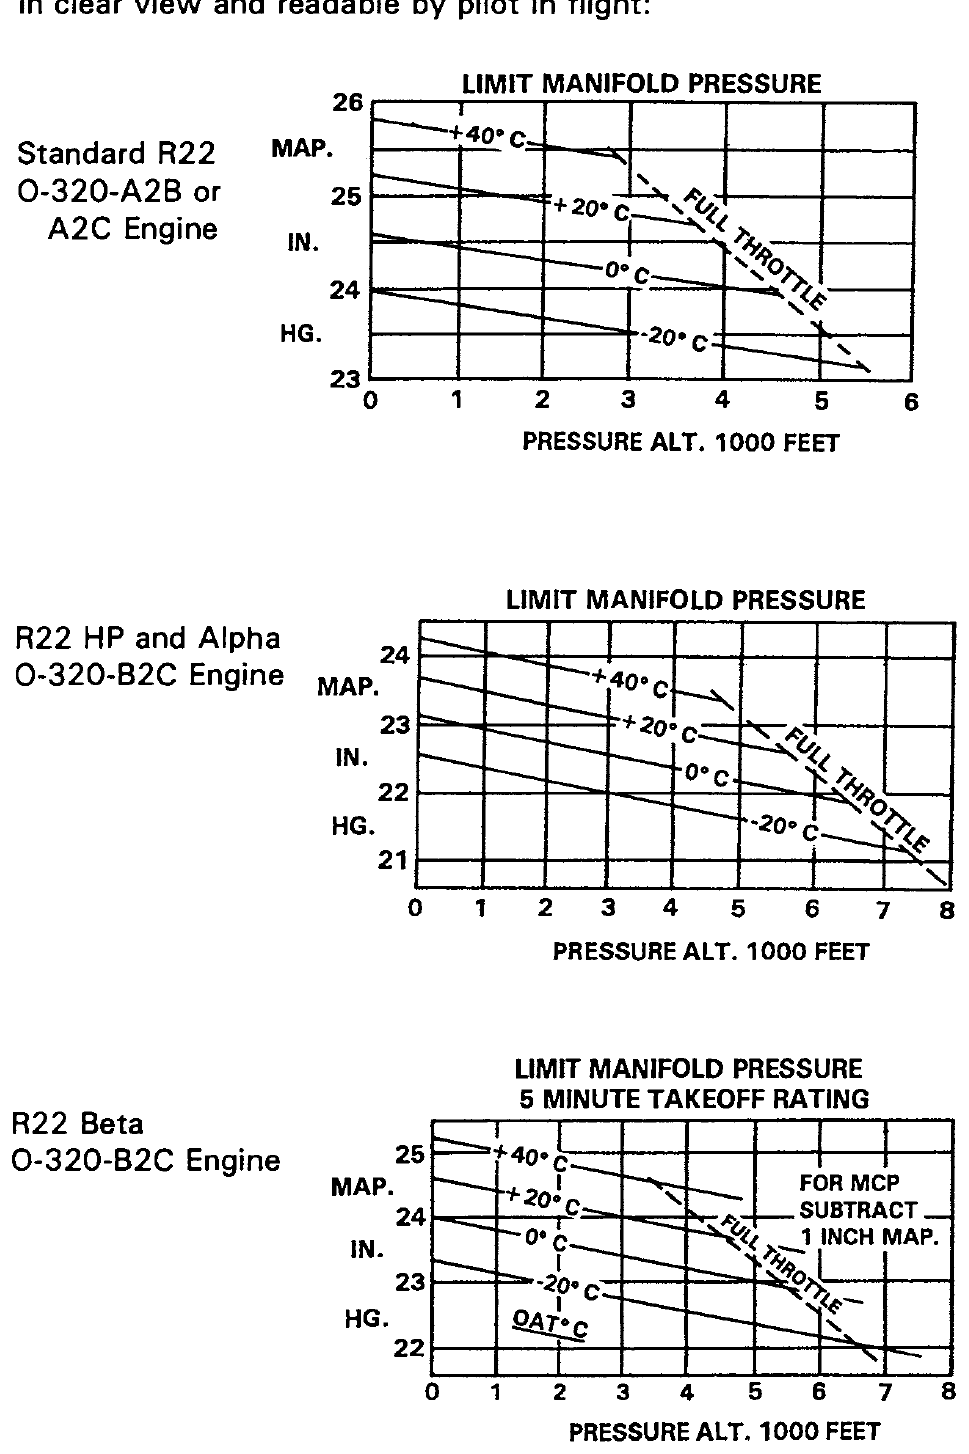
\includegraphics[width=.78\linewidth]{assets/poh/map-o320.png}
\caption{Letreros de límite de presión de admisión en función de la altitud de presión y la OAT. Arriba: R22 Standard (O-320-A2B o -A2C). Al centro: R22 HP y Alpha (O-320-B2C). Abajo: R22 Beta (O-320-B2C), gráfico de potencia de despegue de 5 minutos; para MCP, reste 1~inHg de MAP. Las líneas discontinuas marcan la condición de acelerador completamente abierto (\emph{full throttle}).}
\label{fig:map-o320}
\end{figure}

\begin{table}[htbp]
\centering\small
\caption{R22 Beta II (O-360-J2A): límite de presión de admisión en inHg, potencia máxima continua. Para la potencia máxima de despegue (5 min) sume 0,9~inHg.}
\label{tab:map-beta2}
\begin{tabular}{@{}lccccccc@{}}
\toprule
Alt. presión & \multicolumn{7}{c}{OAT (°C)} \\
\cmidrule(l){2-8}
(ft) & $-20$ & $-10$ & 0 & 10 & 20 & 30 & 40 \\
\midrule
NM (SL) & 21,5 & 21,8 & 22,1 & 22,3 & 22,6 & 22,9 & 23,2 \\
2000 & 21,1 & 21,4 & 21,6 & 21,9 & 22,2 & 22,5 & 22,8 \\
4000 & 20,7 & 21,0 & 21,2 & 21,5 & 21,8 & 22,0 & 22,3 \\
6000 & 20,3 & 20,6 & 20,8 & 21,1 & 21,3 & 21,6 & 21,9 \\
8000 & 19,9 & 20,2 & 20,4 & 20,7 & 20,9 & \multicolumn{2}{c}{\footnotesize acelerador a fondo} \\
\bottomrule
\end{tabular}
\end{table}

\subsection{Velocidad que nunca debe excederse}
\label{sec:letreros-vne}

\begin{figure}[htbp]
\centering
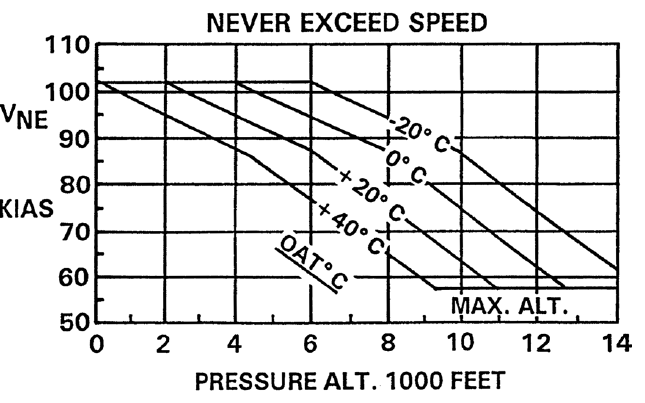
\includegraphics[width=.82\linewidth]{assets/poh/vne-grafico.png}
\caption{\textsc{v}\textsubscript{NE} (KIAS) en función de la altitud de presión y la OAT, para todos los R22 excepto el Beta II. La línea horizontal inferior marca la altitud máxima.}
\end{figure}

\begin{table}[htbp]
\centering\small
\caption{R22 Beta II: \textsc{v}\textsubscript{NE} en KIAS según altitud de presión y OAT. ``Sin vuelo'' (s/v) indica condiciones fuera de la envolvente aprobada.}
\begin{tabular}{@{}lccccccc@{}}
\toprule
Alt. presión & \multicolumn{7}{c}{OAT (°C)} \\
\cmidrule(l){2-8}
(ft) & $-20$ & $-10$ & 0 & 10 & 20 & 30 & 40 \\
\midrule
NM (SL) & 102 & 102 & 102 & 102 & 102 & 102 & 102 \\
2000 & 102 & 102 & 102 & 102 & 102 & 99 & 96 \\
4000 & 102 & 102 & 102 & 98 & 94 & 91 & 87 \\
6000 & 102 & 98 & 94 & 90 & 87 & 82 & 77 \\
8000 & 94 & 90 & 86 & 80 & 75 & 69 & 64 \\
10000 & 86 & 80 & 74 & 68 & 62 & 57 & s/v \\
12000 & 74 & 67 & 61 & \multicolumn{4}{c}{sin vuelo} \\
14000 & 61 & \multicolumn{6}{c}{sin vuelo} \\
\bottomrule
\end{tabular}
\end{table}

\subsection{Letreros de combustible}

Junto a la tapa del tanque principal, uno de los siguientes:
\begin{itemize}
\item \textsf{FUEL --- 100 OCT MIN GRADE AVIATION GASOLINE} (gasolina de aviación, grado mínimo 100 octanos);
\item \textsf{FUEL --- 91/96 MIN GRADE AVIATION GASOLINE};
\item \textsf{FUEL --- AVIATION GASOLINE -- GRADE 100LL OR SEE PILOT'S HANDBOOK};
\item en los R22 con motor O-320-A2B o -A2C puede figurar \textsf{FUEL --- 80/87 MIN GRADE AVIATION GASOLINE}.
\end{itemize}

Junto a la tapa del tanque auxiliar: \textsf{AUX FUEL} con las mismas tres alternativas (100 octanos, 91/96 o 100LL ``o ver el manual del piloto'').

Junto a la válvula de corte: \textsf{FUEL ON / OFF}.

Junto al indicador del tanque principal: \textsf{16.9 US GAL} (tanque con vejiga) o \textsf{19.2 US GAL} (tanque de aluminio). Junto al indicador del auxiliar: \textsf{AUX 9.4 US GAL} (vejiga) o \textsf{AUX 10.5 US GAL} (aluminio).

\subsection{Otros letreros}

\begin{itemize}
\item A la vista de ambos ocupantes: \textsf{NO SMOKING} (prohibido fumar).
\item A la vista del piloto (Alpha, Beta y Beta II con batería trasera): \textsf{MINIMUM SOLO PILOT WEIGHT 130 LB (135 LB WITH FULL AUX FUEL)} --- peso mínimo del piloto solo 130~lb (135~lb con el tanque auxiliar lleno) --- o bien \textsf{SEE PILOT'S HANDBOOK FOR SOLO PILOT WEIGHT LESS THAN 135 LB (61 KG)}.
\item A la vista del piloto: \textsf{THIS ROTORCRAFT APPROVED FOR DAY AND NIGHT VFR OPERATIONS} y \textsf{LOW-G PUSHOVERS PROHIBITED}.
\item En el cíclico izquierdo: \textsf{SOLO FROM RIGHT SEAT ONLY} (vuelo solo únicamente desde el asiento derecho).
\item En o junto a los colectivos: \textsf{NO STOWAGE --- KEEP AREA CLEAR} (no guardar objetos; mantener el área despejada).
\item Dentro de cada compartimiento de equipaje: \textsf{CAUTION --- DO NOT EXCEED ANY OF THE FOLLOWING: COMPARTMENT CAPACITY 50 LB MAX; COMBINED SEAT PLUS COMPARTMENT 240 LB MAX; ROTORCRAFT GROSS WEIGHT LIMIT. SEE ROTORCRAFT FLIGHT MANUAL FOR ADDITIONAL INSTRUCTIONS.}
\item En el indicador de temperatura del carburador: \textsf{CAUTION --- BELOW 18 IN. MP, IGNORE GAGE \& APPLY FULL CARB HEAT} (bajo 18~inHg de MAP, ignore el indicador y aplique calefacción total).
\item Junto al control de calefacción, si está instalado: \textsf{IN CASE OF ENGINE FIRE PUSH HEATER CONTROL TO OFF} (en caso de fuego de motor, empuje el control de calefacción a OFF).
\end{itemize}

\section{Información según la AD 95-26-04 de la FAA}
\label{sec:ad9526-lim}

Las siguientes limitaciones (1 a 3) deben observarse salvo que el piloto que manipula los controles haya registrado 200 o más horas de vuelo en helicópteros, de las cuales al menos 50 en el R22, y haya completado el entrenamiento de concientización especificado en el SFAR N.º 73 (27 de febrero de 1995).

\begin{pasos}
\item Prohibido el vuelo con viento en superficie superior a 25~kt, incluidas las ráfagas.
\item Prohibido el vuelo cuando la diferencia entre viento medio y ráfagas supere 15~kt.
\item Prohibido continuar el vuelo en turbulencia moderada, severa o extrema.
\end{pasos}

Al encontrar inadvertidamente turbulencia moderada, severa o extrema, ajuste la velocidad de avance entre 60~KIAS y 0,7\,\textsc{v}\textsubscript{NE}, pero no menos de 57~KIAS.

\begin{nota}
Turbulencia moderada es la que causa (1) cambios de altitud o actitud, (2) variaciones de la velocidad indicada y (3) que los ocupantes sientan una clara tensión contra los cinturones. Esta AD es emitida por la FAA y aplica a helicópteros matriculados en los EE.\,UU.
\end{nota}
